\documentclass{classrep}
\usepackage[utf8]{inputenc}
\usepackage{graphicx}
\usepackage{color}
\usepackage{caption} % opcjonalnie, dla lepszego formatowania

\DeclareUnicodeCharacter{00A0}{~}

\studycycle{Informatyka, studia dzienne, inż I st.}
\coursesemester{IV}

\coursename{Sztuczna inteligencja i systemy ekspertowe}
\courseyear{2024/2025}

\courseteacher{Dr. inż. Krzysztof Lichy}
\coursegroup{wtorek, 12:00}

\author{
  \studentinfo{Mikołaj Pawłoś}{258681} \and
  \studentinfo{Emilia Szczerba}{251643}
}

\title{Zadanie drugie: Poprawa lokalizacji UWB przy pomocy sieci neuronowych}

\begin{document}
\maketitle

\section{Cel}
 {Zaprojektowanie i zaimplementowanie sieci neuronowej,
  która pozwoli na korygowanie błędów uzyskanych z systemu pomiarowego.}


\section{Wprowadzenie}
\paragraph{}

\subsection{Sieć neuronowa}
\textbf{Sieć neuronowa} (znana również jako \textit{sztuczna sieć neuronowa},
w skrócie \textbf{NN} lub \textbf{ANN})
to model obliczeniowy inspirowany strukturą i funkcjami biologicznych sieci neuronowych.
Sieć neuronowa składa się z połączonych jednostek lub węzłów, zwanych \textbf{sztucznymi neuronami}, które luźno odwzorowują neurony w mózgu.
\paragraph{}
\textbf{Neurony} są połączone \textbf{krawędziami}, które odwzorowują synapsy w mózgu. Każdy sztuczny neuron odbiera sygnały od połączonych z nim neuronów, przetwarza je, a następnie wysyła sygnał do kolejnych połączonych neuronów.
\paragraph{}
„\textbf{Sygnał}” ma postać liczby rzeczywistej, a wyjście neuronu obliczane jest
za pomocą pewnej nieliniowej funkcji sumy jego wejść, zwanej \textbf{funkcją aktywacji}.
\paragraph{}
Siła sygnału w każdym połączeniu jest określana przez \textbf{wagę}, która jest dostosowywana podczas procesu uczenia.

Zazwyczaj neurony grupowane są w \textbf{warstwy}. Różne warstwy mogą wykonywać różne transformacje danych wejściowych.
Sygnały przepływają od pierwszej warstwy (\textit{warstwa wejściowa}) do ostatniej (\textit{warstwa wyjściowa}),
przechodząc być może przez kilka warstw pośrednich (\textit{warstw ukrytych}).
Sieć nazywa się \textbf{głęboką siecią neuronową}, jeśli zawiera co najmniej dwie warstwy ukryte.

\begin{figure}[h!]
	\centering
	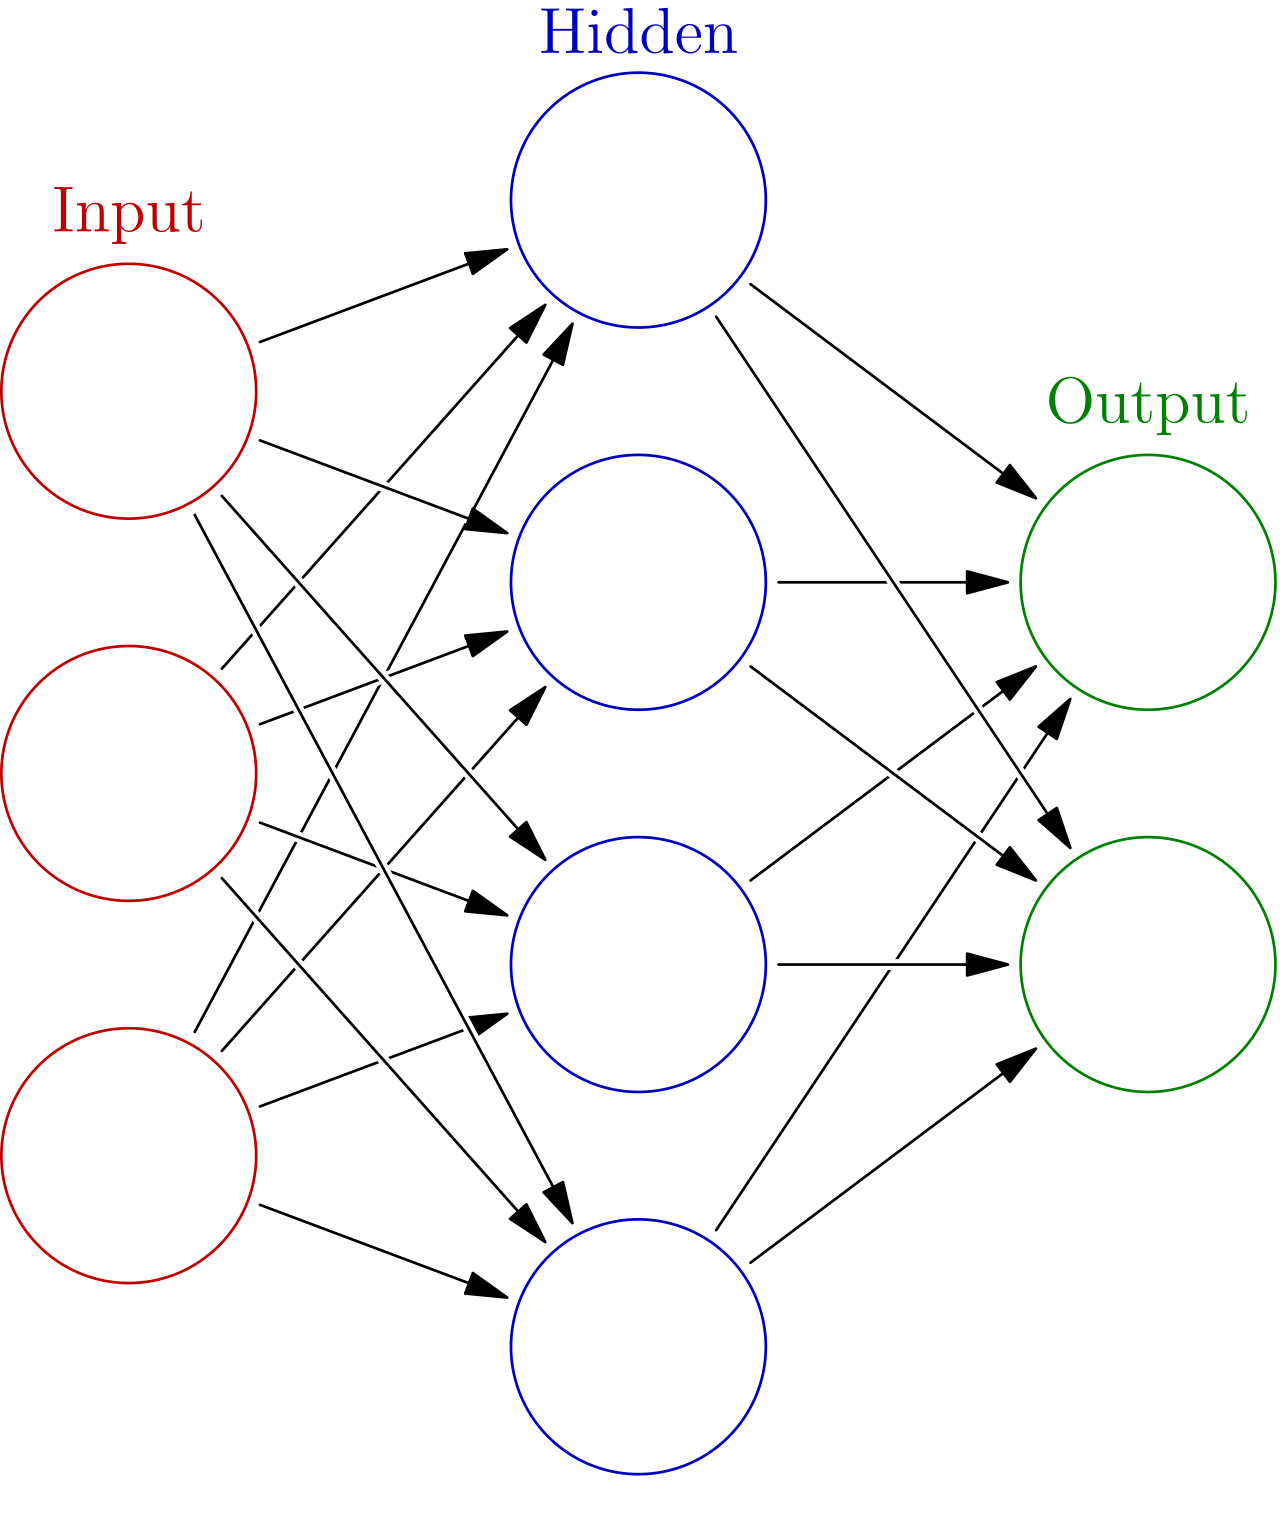
\includegraphics[scale=0.2]{nn.png}
	\caption{Schemat przykładowej sieci neuronowej}
	\label{fig:nn}
\end{figure}

Sztuczne sieci neuronowe są wykorzystywane w różnych zadaniach, takich jak \textit{modelowanie predykcyjne}, \textit{sterowanie adaptacyjne} czy \textit{rozwiązywanie problemów z zakresu sztucznej inteligencji}. Potrafią uczyć się na podstawie doświadczenia i wyciągać wnioski z złożonych i pozornie niepowiązanych danych.
\clearpage{}
\subsection{Systemy lokalizacji UWB}
Technologia \textbf{Ultra-Wideband (UWB)} wykorzystuje krótkie impulsy radiowe o bardzo szerokim paśmie częstotliwości (powyżej 500 MHz), co umożliwia precyzyjny pomiar odległości między nadajnikiem a odbiornikiem. Główną zaletą UWB jest wysoka odporność na zakłócenia wielodrogowe (\textit{multipath}) oraz możliwość osiągnięcia dokładności lokalizacji rzędu \textbf{kilku centymetrów}.

Kluczowe metody lokalizacji w UWB obejmują:
\begin{itemize}
	\item \textbf{TOA (Time of Arrival)} -- pomiar czasu dotarcia sygnału,
	\item \textbf{TDOA (Time Difference of Arrival)} -- różnica czasu dotarcia do wielu odbiorników,
	\item \textbf{RSSI (Received Signal Strength Indication)} -- pomiar mocy sygnału (mniej precyzyjny niż TOA/TDOA).
\end{itemize}

\begin{figure}[h!]
	\centering
	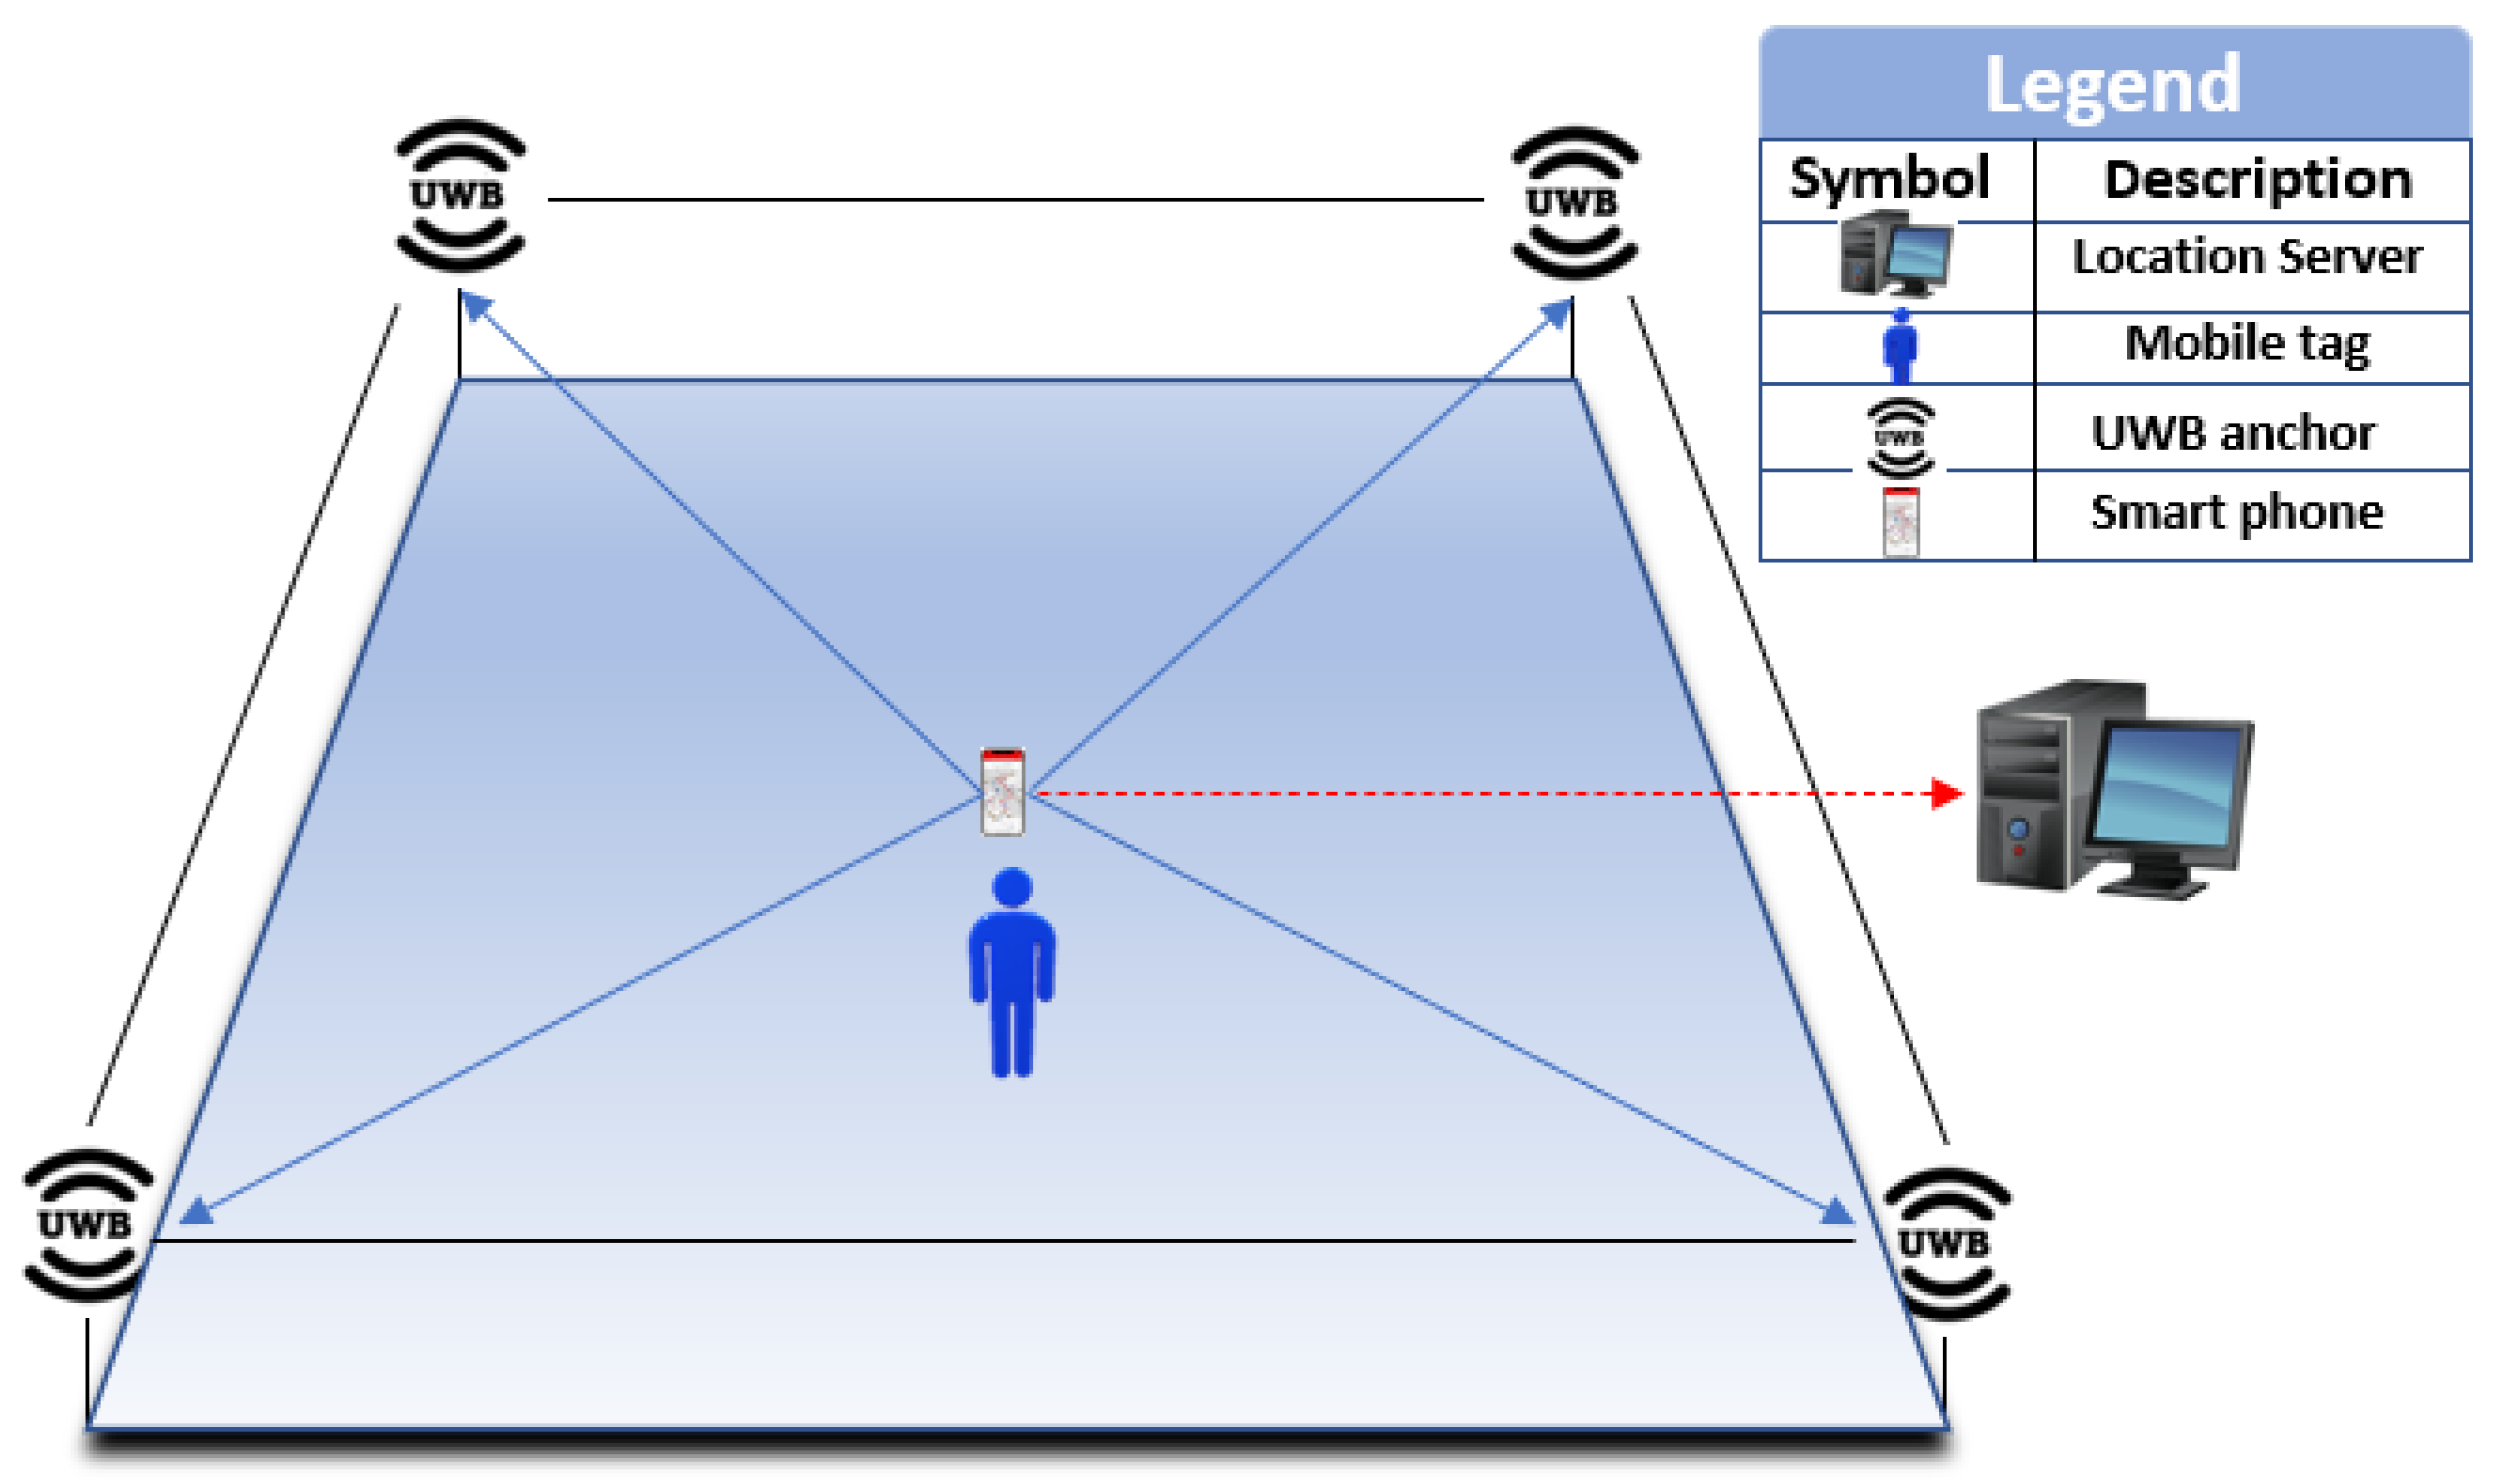
\includegraphics[scale=0.1]{uwb.png}
	\caption{przykładowy system lokalizacji UWB}
	\label{fig:uwb}
\end{figure}

\noindent Ograniczenia systemów UWB obejmują:
\begin{itemize}
	\item Wpływ przeszkód fizycznych (np. ściany) na propagację sygnału,
	\item Błędy synchronizacji czasowej między urządzeniami,
	\item Zależność od konfiguracji środowiska (np. rozmieszczenie anchorów).
\end{itemize}
\clearpage{}
\subsection{Uczenie sieci neuronowej}
Proces uczenia sieci neuronowej polega na dostosowywaniu wag połączeń między neuronami w celu minimalizacji funkcji straty (\textit{loss function}), która mierzy różnicę między przewidywaniami modelu a rzeczywistymi wartościami. Kluczowe etapy tego procesu obejmują:

\begin{itemize}
	\item \textbf{Propagację wprzód} (\textit{forward propagation}) -- obliczenie wyjścia sieci na podstawie danych wejściowych i aktualnych wag.
	\item \textbf{Obliczenie funkcji straty} -- np. średni błąd kwadratowy (MSE) dla zadań regresji:
	      \begin{equation}
		      \text{MSE} = \frac{1}{n} \sum_{i=1}^{n} (y_i - \hat{y}_i)^2,
	      \end{equation}
	      gdzie \( y_i \) to wartość rzeczywista, a \( \hat{y}_i \) to przewidywana wartość.
	\item \textbf{Propagację wsteczną} (\textit{backpropagation}) -- obliczenie gradientów funkcji straty względem wag i ich aktualizacja przy użyciu optymalizatora (np. Adam, SGD).
\end{itemize}

\noindent W projekcie zastosowano dodatkowe techniki poprawiające uczenie, takie jak:
\begin{itemize}
	\item \textbf{Wczesne zatrzymanie} (\textit{early stopping}) -- przerwanie uczenia, gdy błąd na zbiorze walidacyjnym przestaje maleć.
	\item \textbf{Normalizacja danych} -- przekształcenie cech do podobnego zakresu wartości (np. przy użyciu StandardScaler).
\end{itemize}
\clearpage{}
\section{Opis implementacji}

Zadanie zostało wykonane przy użyciu języka \textbf{Python3}, z wykorzystaniem następujących bibliotek:

\begin{itemize}
	\item \texttt{Matplotlib}
	\item \texttt{Numpy}
	\item \texttt{PyTorch}
	\item \texttt{scikit-learn}
\end{itemize}

Projekt został podzielony na następujące pliki:

\begin{enumerate}
	\item \texttt{DataLoader.py} – moduł odpowiedzialny za wczytywanie, filtrowanie i wstępne przetwarzanie danych pomiarowych z plików Excel.

	\item \texttt{NeuralNetworkModel.py} – główny moduł modelu uczenia maszynowego opartego na sieci neuronowej. Odpowiada za tworzenie, trenowanie, testowanie i zapisywanie modelu, z uwzględnieniem mechanizmów detekcji outlierów i normalizacji danych.

	\item \texttt{OutlierDetector.py} – moduł odpowiedzialny za identyfikację obserwacji odstających w danych wejściowych. Wspiera różne metody detekcji, m.in. oparte na odległości Mahalanobisa czy odchyleniu standardowym.

	\item \texttt{main.py} – plik uruchomieniowy, zawierający konfigurację eksperymentów, wczytywanie danych, inicjalizację modelu oraz zapisywanie wyników i metryk. Stanowi punkt wejścia do całego systemu.

\end{enumerate}

\clearpage{}
\subsection{Plik \texttt{DataLoader.py}}

Moduł \texttt{DataLoader.py} odpowiada za ładowanie oraz wstępne przetwarzanie danych pomiarowych wykorzystywanych w procesie uczenia i testowania modeli.
Główne zadania realizowane przez ten moduł to:
\begin{itemize}
	\item automatyczne lokalizowanie folderów z danymi wejściowymi (statycznymi i dynamicznymi),
	\item odczyt danych z plików Excel (\texttt{.xlsx}) znajdujących się w podfolderach \texttt{F8} i \texttt{F10},
	\item wstępne czyszczenie danych – usuwanie pustych wierszy,
	\item selekcja i ekstrakcja cech sensorycznych z kolumn (np. akcelerometr, żyroskop, ciśnienie, kwaterniony),
\end{itemize}
\paragraph{}
Dane są dzielone na zbiór treningowy (pochodzący z plików statycznych) oraz testowy (z plików dynamicznych), a następnie przekształcane do postaci numerycznych macierzy przy pomocy biblioteki NumPy.
Moduł ten stanowi fundament do dalszych etapów analizy i modelowania, zapewniając jednolite i ustandaryzowan

\noindent\rule{8cm}{0.4pt}

\subsection{Plik \texttt{NeuralNetworkModel.py}}

Plik \texttt{NeuralNetworkModel.py} zawiera kompletną implementację modelu sieci neuronowej zaprojektowanej z myślą o regresji wielowymiarowej oraz automatycznej detekcji i eliminacji obserwacji odstających (ang. outliers).

\paragraph{}
Moduł składa się z dwóch głównych klas:
\begin{itemize}
	\item \texttt{NeuralNetwork} – definiuje architekturę wielowarstwowej sieci neuronowej typu \textit{feedforward} z konfigurowalną liczbą warstw ukrytych, funkcją aktywacji i mechanizmem \texttt{Dropout}.
	\item \texttt{EnhancedNeuralNetworkModel} – klasa wyższego poziomu integrująca funkcje uczenia, walidacji, normalizacji danych, predykcji oraz obsługi danych odstających przy użyciu zewnętrznego modułu \texttt{OutlierDetector}.
\end{itemize}

\paragraph{}
Model wspiera różne optymalizatory (Adam, SGD), posiada wbudowany mechanizm \textit{early stopping}, adaptacyjny harmonogram uczenia (\texttt{ReduceLROnPlateau}) oraz możliwość zapisu i odczytu wag modelu (zarówno w formacie binarnym \texttt{.pt}, jak i w postaci tabeli CSV).

Trening odbywa się z użyciem biblioteki PyTorch, a dane wejściowe są wstępnie przeskalowywane za pomocą standaryzacji (\texttt{StandardScaler}) z biblioteki \texttt{scikit-learn}. Proces walidacji może być przeprowadzony na osobnym zbiorze lub automatycznie podzielony z danych treningowych.

Architektura modelu jest w pełni parametryzowana: użytkownik może zdefiniować liczbę neuronów wejściowych, wyjściowych, strukturę warstw ukrytych, liczbę epok, współczynnik uczenia, funkcję aktywacji, metodę detekcji outlierów, a także urządzenie obliczeniowe (\texttt{CPU} lub \texttt{GPU}).

\subsubsection*{Architektura modelu bez eliminacji wartości odstających}

Po wielu eksperymentach, metodą prób i błędów, zdecydowaliśmy się na zastosowanie poniższej architektury sieci neuronowej.

\begin{itemize}
	\item Liczba warstw ukrytych: 3
	\item Liczba neuronów w warstwach: 256, 128, 64
	\item Funkcja aktywacji: ReLU (Rectified Linear Unit)
	\item Liczba neuronów wyjściowych: 2
	\item Liczba epok: 300
	\item Rozmiar partii (batch size): 128
	\item Współczynnik uczenia (learning rate): 0{,}001
\end{itemize}

\clearpage{}

\subsection{Plik \texttt{main.py}}

\subsubsection*{Główna funkcja \texttt{main()}}

Funkcja \texttt{main()} zawiera pełny pipeline systemu korekcji i składa się z następujących etapów:

\begin{enumerate}
	\item Wczytanie danych uczących i testowych przy pomocy klasy \texttt{DataLoader}.

	\item Utworzenie i trenowanie dwóch modeli sieci neuronowych:
	      \begin{itemize}
		      \item bez usuwania wartości odstających (outlierów),
		      \item z eliminacją outlierów przy użyciu złożonej metody detekcji.
	      \end{itemize}

	\item Przewidywanie błędów przez modele, ich odejmowanie od danych wejściowych oraz ocena skuteczności korekcji.

	\item Obliczenie metryk błędu dla każdego z podejść oraz zapis wyników do pliku tekstowego i arkusza kalkulacyjnego.

	\item Generowanie wykresów i zapis danych dystrybuanty błędów do plików \texttt{.xlsx}.

	\item Zapis wytrenowanych modeli w formacie PyTorch (\texttt{.pth}).
\end{enumerate}

\subsubsection*{Efekty działania i generowane pliki}

W wyniku działania programu generowane są:

\begin{itemize}
	\item Wykresy: \texttt{training\_history.png}, \texttt{error\_analysis\_*.png},
	\item Modele: \texttt{model\_bez\_outlierow.pth}, \texttt{model\_z\_outlierami.pth},
	\item Dane wyjściowe: \texttt{dystrybuanta\_*.xlsx}, \texttt{wyniki\_szczegolowe.xlsx},

	      \texttt{raport\_podsumowanie.txt}.
\end{itemize}

Plik ten stanowi główny komponent praktyczny systemu korekcji błędów i integruje cały proces od wczytania danych po ocenę skuteczności modelu.

\section{Materiały i metody}
 {\color{blue}
  W tym miejscu należy opisać, jak przeprowadzone zostały wszystkie badania,
  których wyniki i dyskusja zamieszczane są w dalszych sekcjach. Opis ten
  powinien być na tyle dokładny, aby osoba czytająca go potrafiła wszystkie
  przeprowadzone badania samodzielnie powtórzyć w celu zweryfikowania ich
  poprawności. Przy opisie należy odwoływać się i stosować do
  opisanych w sekcji drugiej wzorów i oznaczeń, a także w jasny sposób opisać
  cel konkretnego testu. Najlepiej byłoby wyraźnie wyszczególnić (ponumerować)
  poszczególne eksperymenty tak, aby łatwo było się do nich odwoływać dalej.}

\clearpage{}
\section{Wyniki} {
  \begin{figure}[h!]
	  \centering
	  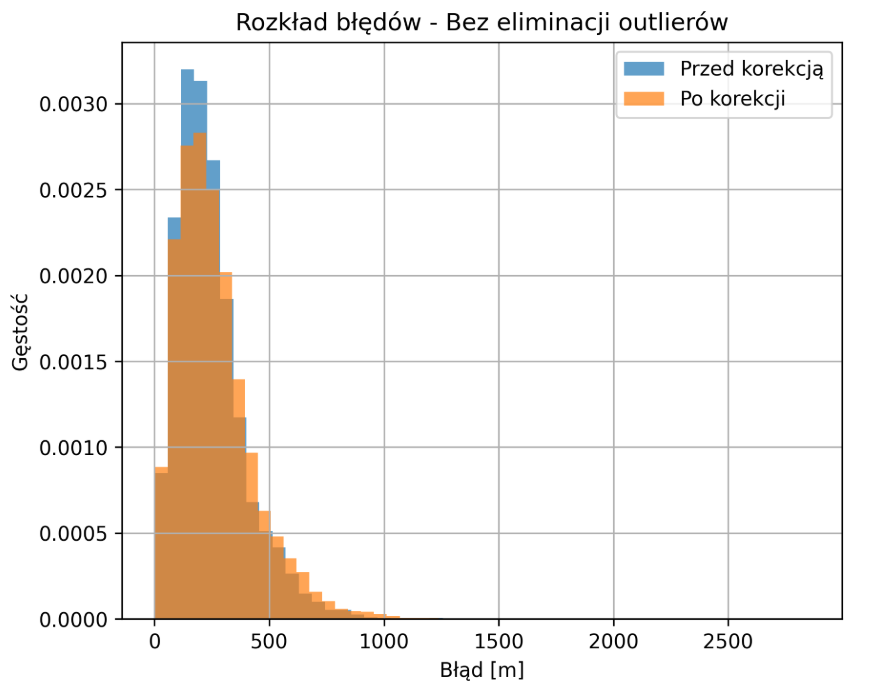
\includegraphics[scale=0.40]{gestoscBl.png}
	  \caption{Rozkład błędów po korekcji}
	  \label{fig:density}
  \end{figure}
  \begin{figure}[h!]
	  \centering
	  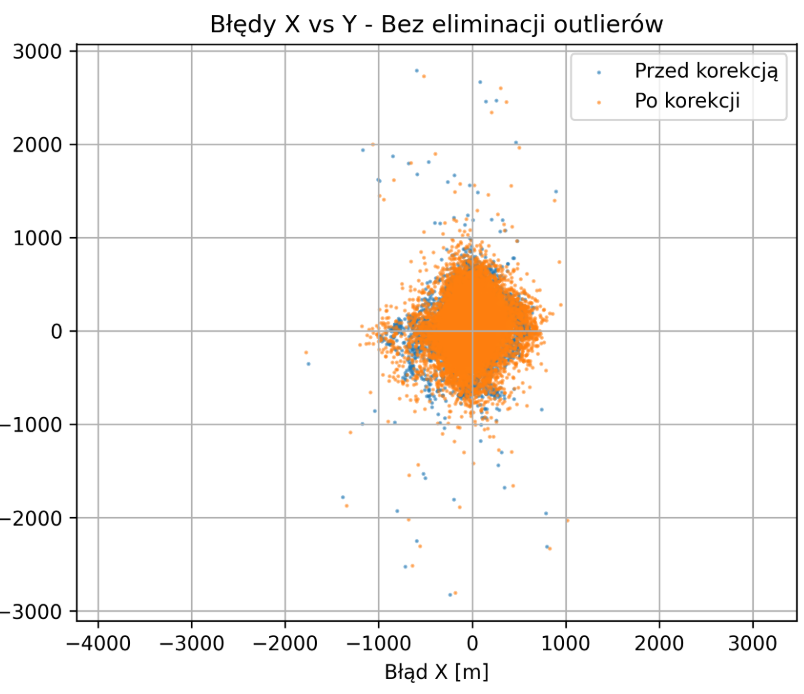
\includegraphics[scale=0.40]{rozkladBl.png}
	  \caption{Rozproszenie błedów x, y}
	  \label{fig:błedyXY}
  \end{figure}
  \begin{figure}[h!]
	  \centering
	  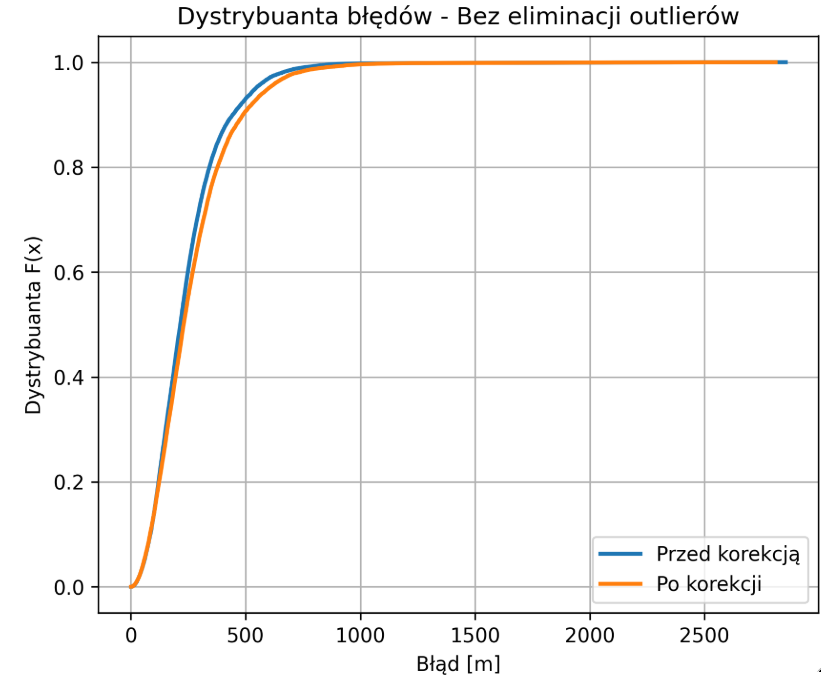
\includegraphics[scale=0.40]{dystrb.png}
	  \caption{zmiana dystrybuanty}
	  \label{fig:dystrybuanta}
  \end{figure}
  \begin{table}[ht]
	  \centering
	  \caption{Wagi cech sieci neuronowej}
	  \begin{tabular}{|c|l|r|}
		  \hline
		  \textbf{\#} & \textbf{cecha}                             & \textbf{waga} \\
		  \hline
		  1           & data\_\_tagData\_\_linearAcceleration\_\_y & 0.159497      \\
		  2           & data\_\_tagData\_\_quaternion\_\_x         & 0.150790      \\
		  3           & data\_\_tagData\_\_linearAcceleration\_\_x & 0.143811      \\
		  4           & data\_\_tagData\_\_quaternion\_\_y         & 0.143303      \\
		  5           & data\_\_tagData\_\_magnetic\_\_x           & 0.137812      \\
		  6           & data\_\_tagData\_\_quaternion\_\_z         & 0.132061      \\
		  7           & data\_\_tagData\_\_magnetic\_\_z           & 0.129842      \\
		  8           & data\_\_tagData\_\_quaternion\_\_w         & 0.121032      \\
		  9           & data\_\_tagData\_\_pressure                & 0.120398      \\
		  10          & data\_\_tagData\_\_magnetic\_\_y           & 0.111724      \\
		  11          & data\_\_tagData\_\_gyro\_\_z               & 0.067959      \\
		  12          & data\_\_tagData\_\_linearAcceleration\_\_z & 0.067480      \\
		  13          & data\_\_tagData\_\_gyro\_\_y               & 0.047070      \\
		  14          & data\_\_tagData\_\_gyro\_\_x               & 0.041198      \\
		  \hline
	  \end{tabular}
	  \label{tab:nn_weights}
  \end{table}
 }
\clearpage{}

\section{Dyskusja}
Z uzyskanych wyników widzimy że rozkład błędów stał się bardziej "precyzyjny" (Rys. 4),
oraz że zmniejszyła się gęstość występowania błędów w zakresie ok. 0 - 350 (Rysunek 3).
Dystrybuanta ogólnie zmieniła się negatywnie z jedynie nieznaczną poprawą na zakresie podanym wyżej.

\section{Wnioski}
 {\color{blue}
  W tej, przedostatniej, sekcji należy zamieścić podsumowanie najważniejszych
  wniosków z sekcji poprzedniej. Najlepiej jest je po prostu wypunktować. Znów,
  tak jak poprzednio, najistotniejsze są wnioski o charakterze uniwersalnym.}

\begin{thebibliography}{0}
	\bibitem{nn} Wikipedia contributors. "Neural network (machine learning)."
	Wikipedia, The Free Encyclopedia. Wikipedia, The Free Encyclopedia,
	2025.

	\bibitem{uwb} Wikipedia contributors. (2025, May 25). \textit{Ultra-wideband}.
	In Wikipedia, The Free Encyclopedia. 2025

\end{thebibliography}

{\color{blue}
Na końcu należy obowiązkowo podać cytowaną w sprawozdaniu literaturę, z której
grupa korzystała w trakcie prac nad zadaniem.}

\end{document}
